\documentclass{report}
% \usepackage[T5]{fontenc}
\usepackage[utf8]{inputenc}
\usepackage{mathtools}
% \usepackage{times}
\usepackage{amssymb}
\usepackage{longtable}
\renewcommand{\arraystretch}{1.5}

% \usepackage[a4paper, left=1.18in,top=0.79in,right=0.79in,bottom=0.79in,bindingoffset=0cm]{geometry}
\usepackage[a4paper, bindingoffset=0cm]{geometry}
% \usepackage[a4paper]{geometry}
\usepackage{graphicx}
\usepackage{tikz}
\usetikzlibrary{calc}
% \usepackage[skip=10pt plus1pt, indent=1.25cm]{parskip}
\usepackage{indentfirst}
\usepackage{float}
% \usepackage[font=large]{caption}
\usepackage{listings}
\usepackage{xcolor}

\definecolor{codegreen}{rgb}{0,0.6,0}
\definecolor{codegray}{rgb}{0.5,0.5,0.5}
\definecolor{codepurple}{rgb}{0.58,0,0.82}
\definecolor{backcolour}{rgb}{0.95,0.95,0.92}

\lstdefinestyle{mystyle}{
    backgroundcolor=\color{backcolour},   
    commentstyle=\color{codegreen},
    keywordstyle=\color{magenta},
    numberstyle=\tiny\color{codegray},
    stringstyle=\color{codepurple},
    basicstyle=\ttfamily\footnotesize,
    breakatwhitespace=false,         
    breaklines=true,                 
    captionpos=b,                    
    keepspaces=true,                 
    numbers=left,                    
    numbersep=5pt,                  
    showspaces=false,                
    showstringspaces=false,
    showtabs=false,                  
    tabsize=2
}

\lstset{style=mystyle}
\usepackage{subcaption}
\newcommand\HRule{\rule{\textwidth}{1pt}}

\newtheorem{definition}{Definition}[chapter]
\usepackage[printonlyused,withpage]{acronym}
\usepackage[backend=biber,style=numeric-comp, sorting=none]{biblatex}
\renewcommand{\bibfont}{\fontsize{14pt}{18pt}}

% \addbibresource{mybibliography.bib}

\usepackage{titletoc}
\usepackage{titlesec}
% \titlecontents{chapter}
%   [0pt]
%   {}
%   {\bfseries \MakeUppercase{\chaptername}\ \thecontentslabel: \ }
%   {}
%   {\bfseries \titlerule*[0.75em]{.} \contentspage}

% \titleformat{\chapter} %[block]
% {\bfseries\centering}
% {\MakeUppercase{\chaptertitlename}\ \thechapter:}{1em}{\MakeUppercase}

% \titleformat{\section}  % which section command to format
%   {\fontsize{14}{16}\bfseries} % format for whole line
%   {\thesection} % how to show number
%   {1em} % space between number and text
%   {} % formatting for just the text
%   [] % formatting for after the text

% \titleformat{\subsection}  % which section command to format
%   {\fontsize{14}{16}\bfseries} % format for whole line
%   {\thesubsection} % how to show number
%   {1em} % space between number and text
%   {} % formatting for just the text
%   [] % formatting for after the text

% \titleformat{\subsubsection}  % which section command to format
%   {\fontsize{14}{16}\bfseries} % format for whole line
%   {\thesubsection} % how to show number
%   {1em} % space between number and text
%   {} % formatting for just the text
%   [] % formatting for after the text

\titlespacing*{\chapter}{0pt}{-20pt}{0pt}

% \pagenumbering{roman}
\pagenumbering{arabic}


\title{Learn Git the hard way, notes}
\author{Quoc-Quan Truong}
\date{November 2023}

\begin{document}

\maketitle

\newpage
\tableofcontents
\newpage

\chapter{GIT BASIC}

Within the .git folder lay many files, of which the HEAD and the config.

The HEAD file is key: it points to the current branch or commit ID you are currently on within your Git repository.

The config file stores information about your repository's local configuration. For example, the branches and remote repositories your repository is aware of

If you want to look at the history of this repository, then run the git log command

The git status command tells you where the HEAD is pointing at and that if there exists something to commit.

Untracked files are files that Git acknowledges their existances, but are unaware by the repo. To make Git aware of them, the files needs to be added to the repository.

The git add Command
The add command tells Git to start tracking the files in the local index

You have added a file to the index. It is ready to be committed to the repository.

Remember the four stages you looked at before.

You created your file ((1) local changes).
You added/staged it to the index (2).
Still, you have no history! Git has simply been made aware of the file, and you must make a commit to initiate Git's history.

The git commit command
The git commit command tells Git to take a snapshot of all added content at this point.

The git diff command
To see the changes that has happened to the files, use the git diff command.

You can commit changes to files and add at the same time by doing git commit -a

\chapter{CLONE A REPOSITORY}

The git clone command
The git clone command helps you create copies of Git repositories to work on.

The git reset command
The git reset command helps you return to a previous or known state.

\begin{lstlisting}
    git log
\end{lstlisting}

This shows you a default history of the repository. Page through it a few times by hitting space or down. You will see how far it goes back. Hit q to stop viewing it, and return to the command line.


\begin{lstlisting}
    git log --oneline
\end{lstlisting}
Another way to view the log is one line per commit, which is much more concise and useful for many purposes. Obviously, some information is lost here.

\begin{lstlisting}
    git log --oneline --graph
\end{lstlisting}

You've added the --graph flag, and now you get a visual representation of the history. Parsing this graph can be tricky; don't worry about understanding it exactly. But keep it in mind. It is helpful if you ever have to figure out what went on in a repository's past.

\chapter{GIT BRANCHING}

\begin{lstlisting}
    git branch
    git checkout
\end{lstlisting}

This introduction shall discuss in length how branches are created in Git To create a new branch, type in:

\begin{lstlisting} 
    git branch <branch_name> 
\end{lstlisting} 

After typing this, a new branch with name \text{<branch\_name>} will be created. However, the HEAD will still be pointed to the initial branch. You can check it by using git status. To see all branches, execute git branch. Another flag of git log is --decorate. This gives you useful information about the reference names (branches and tags) at various commit points. 

To go on to a branch, type in: 

\begin{lstlisting} 
    git checkout <branch_name> 
\end{lstlisting} 

Another flag of git log is added, the --all flag. --all shows all branches, not just the branch you happen to be on. 

\subsection{Detached HEAD} 

Detaching 

The HEAD pointer can be moved to an arbitrary point. In fact, git checkout does exactly this. You can specify a reference (like master or newfeature) or a specific commit ID. 

For example: 
\begin{lstlisting}
    git checkout e36355ed00ac3af009d7113a9dd281c269a79afd
\end{lstlisting}

The detached HEAD state:

\begin{itemize}
    \item Detached HEAD means that the HEAD pointer is not pointing towards a branch, but to a commit ID.
    \item You can look around, make experimental changes and commit them, and you can discard any commits you make in this state without impacting any branches by performing another checkout.
\end{itemize}
 
\chapter{TAGS} 

Tags are the same as branches, but they do not have history. Tags point to commits, but they do not change. Syntax: 
\begin{lstlisting} 
    git checkout <branch_name> 
    git tag <name_of_tag> # tag where you are. 
\end{lstlisting} 
Or you can tag wherever a branch pointer is pointed at in your repository, even if you are not on it.

\begin{lstlisting} 
    git checkout e36355ed00ac3af009d7113a9dd281c269a79afd 
    git branch -f newfeature 
\end{lstlisting} 

The -f flag means --force. If a branch of newfeature already exists, then Git will not allow you to override it unless you use the -f flag. 

\begin{lstlisting} 
    git checkout master git tag remember_to_tell_bob_to_rewrite_this newfeature 
\end{lstlisting} 

Verify the tags with git tag 

\chapter{Conclusion: Git Branching} A branch is just a pointer 

Remember these points: A branch is a pointer to the end of a line of changes. A tag is a pointer to a single change. HEAD is where your Git repository is right now. Detached HEAD means you are at a commit that has no reference (branch or tag) associated with it.

\chapter{MERGING}

\section{Introduction}

\begin{lstlisting}
    git merge
\end{lstlisting}

In this chapter, you will learn about:
\begin{itemize}
    \item Merge conflicts and how to resolve them
    \item Merges and log histories
\end{itemize}

\subsection{Remembering branches}
You've already covered the basics of branching in the previous chapter. As you will recall, branching gives you the ability to work on parallel streams of development in the same codebase.

\subsection{Merging vs. branching}
In a sense, merging is the opposite of branching. When you merge, you take two separate points in your development tree and fuse them together.

It's important to understand merging, as it's a routine job of a repository maintainer to merge branches together.

It's also really important to take this chapter slowly and make sure you understand every step. It's quite painful to wrap your head around merging properly. But once you do, your Git skills will improve.

\section{Pre - merge}

\begin{figure}[H]
    \centering
    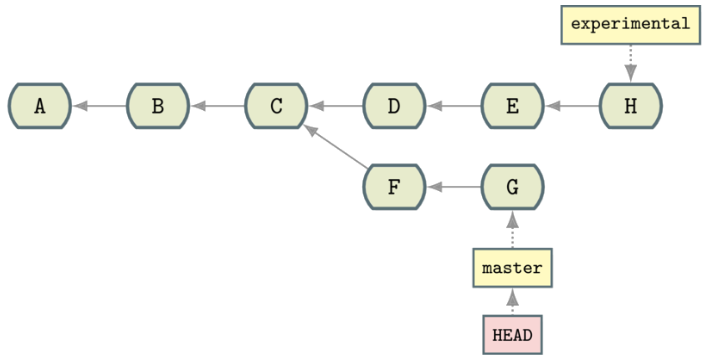
\includegraphics[width=0.5 \linewidth]{Photos/merge-1.png}
    \caption[short]{Pre-merge diagram}
    \label{fig:merge-1} 
\end{figure}

In this particular diagram, the repo is currently positioned at the tip of master \textbf{G}, indicated by the HEAD, which is pointing at \textbf{G}.

\section{Post - merge}

If the `experimental` branch is merged into master with a command:

\begin{lstlisting}
    git merge experimental
\end{lstlisting}

\begin{figure}[H]
    \centering
    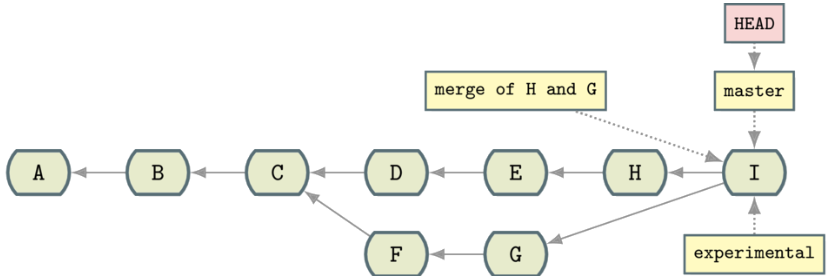
\includegraphics[width=0.5 \linewidth]{Photos/merge-2.png}
    \caption[short]{Post-merge diagram}
    \label{fig:merge-2}
\end{figure}

A new change has been made (\textbf{I}). This change merges together the changes made on experimental with the changes made on master.

\section{Merging, step by step}

\subsection{Step 1: Creating a repository, adding some files, and committing them}

Code:

\begin{lstlisting}
    mkdir -p lgthw_merging
    cd lgthw_merging
    git init
    echo A > file1
    git add file1
    git commit -am 'A'
    echo B >> file1
    git commit -am 'B'
    echo C >> file1
    git commit -am 'C'
\end{lstlisting}

After this, the repository will look like this:

\begin{figure}
    \centering
    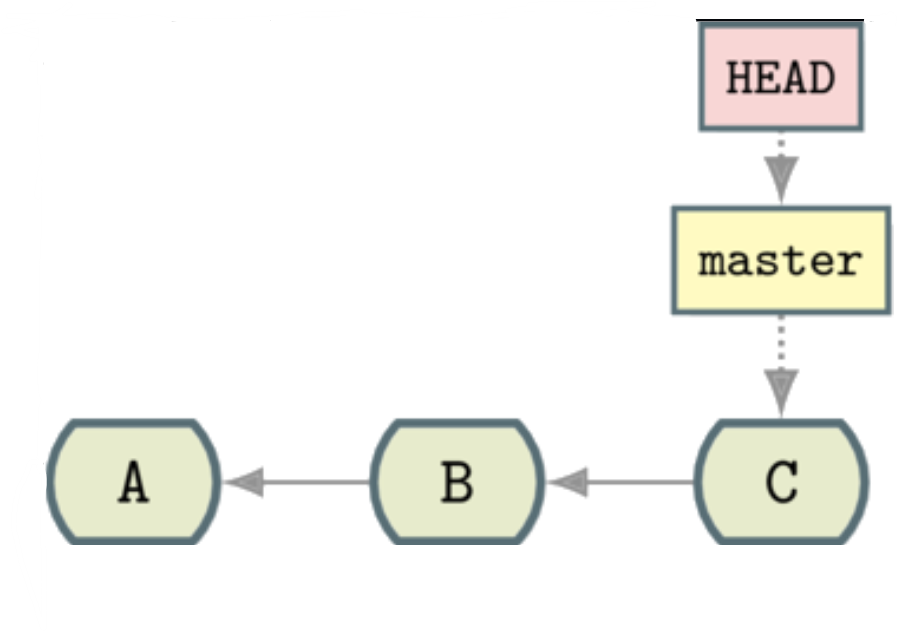
\includegraphics[width=0.5 \linewidth]{Photos/merge-3.png}
    \caption[short]{Repository after step 1}
    \label{fig:merge-3}
\end{figure}

\subsection{Step 2: Creating a branch and checking it out}

Code:

\begin{lstlisting}
    git branch experimental
    git checkout experimental
    git branch
    echo E >> file1
    git commit -am 'E'
    echo H >> file1
    git commit -am 'H'
\end{lstlisting}

After this, the repository will look like this:

\begin{figure}[H]
    \centering
    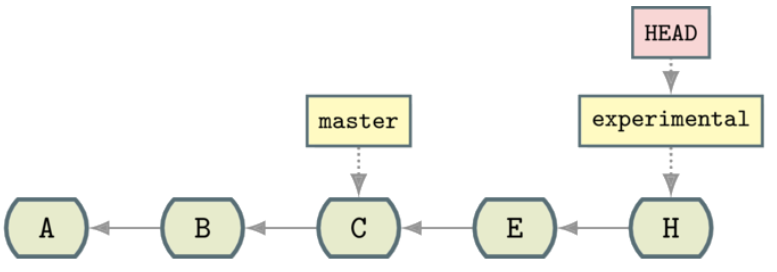
\includegraphics[width=0.5 \linewidth]{Photos/merge-4.png}
    \caption[short]{Repository after step 2}
    \label{fig:merge-4}
\end{figure}

\subsection{Step 3: Checking out master, and making more changes}

Return to master, and make changes D, F and G:

Code:

\begin{lstlisting}
    git checkout master
    echo D >> file1
    git commit -am 'D'
    echo F >> file1
    git commit -am 'F'
    echo G >> file1
    git commit -am 'G'
\end{lstlisting}

After this, the repository will look like this:

\begin{figure}[H]
    \centering
    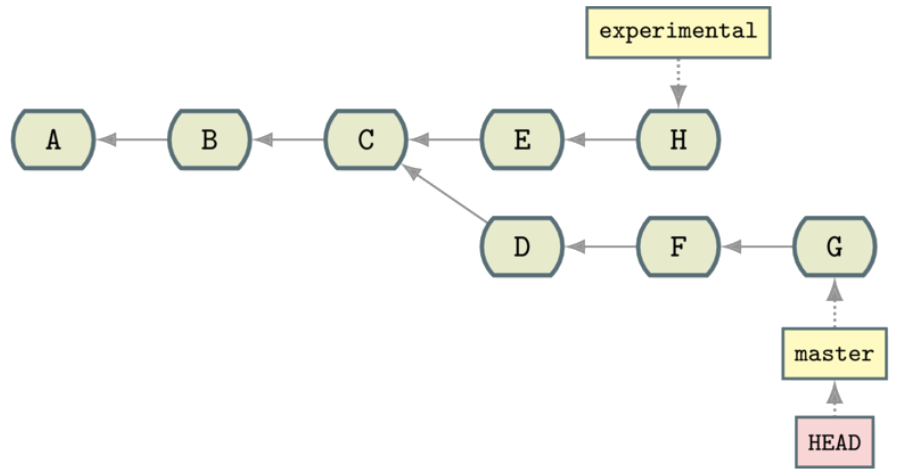
\includegraphics[width=0.5 \linewidth]{Photos/merge-5.png}
    \caption[short]{Repository after step 3}
    \label{fig:merge-5}
\end{figure}

\subsection{Step 4: Attempting to merge the master and experiment branch}

Code:

\begin{lstlisting}
    git merge experimental
\end{lstlisting}

The result of this command is a merge conflict. Git will not allow you to merge the two branches together, because there are conflicting changes on the same line of the same file.

\subsection{Merge conflicts}

When you run a merge, Git looks at the branch you are on (here it is master) and the branch you are merging in (experimental) and works out the first common ancestor. In this case, it's point C, as that's where you branched experimental.

It then takes the changes on the branch that you are merging in from that first common ancestor and applies them to the branch you are on in one go. These changes create a new commit, and the git log graph shows the branches joined back up.

Sometimes the changes made on the branches conflict with one another. That means the changes altered the same lines. In this case, the D, F, and G of the master changed the same lines as the E and H of experimental.

\chapter{Git Stash}

\section{Introduction}

Often when you are working, you want to return to a pristine state but you don't want to lose the work you have done so far. Traditionally, with other source control tools, you've copied files that have changed locally aside, then updated your repository, and then diffed and re-applied the changed files.

Stash away your changes

Git has a concept of the "stash" to store all local changes ready to re-apply at will. You can get very sophisticated with the stash.

\begin{lstlisting}
    [do some work]
    [get interrupted]
    git stash
    [deal with interruption]
    git stash pop
\end{lstlisting}

\section{A hypothetical scenario}

What if I want to work on a new feature, but there's an important update to the code that I need to pull from BitBucket? I don't want to commit my changes, because they're not ready yet. I don't want to lose them either. I want to be able to pull from upstream, and then come back to my current work later. Git stash is the answer.

First, we need to see the what changes we have made locally with \textit{git diff}:

\begin{lstlisting}
    git diff
\end{lstlisting}

After that, we run \textit{git stash} to stash away our changes:

\begin{lstlisting}
    git stash
\end{lstlisting}

A quick \textit{git status} will show that we have no changes:

\begin{lstlisting}
    git status
\end{lstlisting}

What happened to the changes? They are stashed away. You can see them with \textit{git stash list}:

\begin{lstlisting}
    git stash list
\end{lstlisting}

You can also see the graph with \textit{git log}:

\begin{lstlisting}
    git log --graph --oneline --decorate --all
\end{lstlisting}

The resulting return shall give you an overview of what happened:

\begin{lstlisting}
    root@educative:/lgthw_git_stash_1# git log --oneline --graph --decorate --all
    *   24f8db4 (refs/stash) WIP on master: 56a08f1 initial
    |\  
    | * accb0c2 index on master: 56a08f1 initial
    |/  
    * 56a08f1 (HEAD -> master) initial
\end{lstlisting}

Git stash has committed the state of the index and then committed the local change to the refs/stash branch and merged them as a child of the HEAD on a new refs/stash branch.

Don't worry too much about the details yet; it has basically stored all the changes you've made (but not committed), ready to be re-applied.

The stash branch is a special one that is kept local to the current repository. The "commit" message WIP on master and index on master is added automatically.

The master branch is still where it was before you stashed, and the HEAD pointer is pointed at the master branch.

Other work can now be done (in this case, pulling the latest changes from a remote. Remember, we will cover remotes in a later section) without concern for whether it conflicts with those changes.

\section{Retrieving the stash list}

To retrieve the stash list, you can use the \textit{git stash list} command:

\begin{lstlisting}
    git stash list
\end{lstlisting}

\section{Popping stashed work}

Once ready, you can re-apply those changes on the same codebase by running git stash pop:

\begin{lstlisting}
    git stash pop
\end{lstlisting}

It "pops" the zero-numbered change off the stash stack and restores the changes that was stashed, applied to wherever we've ended up.

\subsection{What's a Stack?}
A stack is a computer science concept of a series of items stored in such a way that you can "push" an item to the top of it for any number of times and then "pop" an item off the top until it's empty. When you pop, you only get the most recent item that was pushed on. This means that when you pop your Git stash, you get the most recent one you pushed (which is likely to be what you wanted).

\chapter{Git add interactive}

This chapter will cover the git add -i command and the following topics:

\begin{itemize}
    \item Interactively adding files in Git
    \item Splitting hunks
    \item The difference between staging and committing
\end{itemize}

\section{Recap}

Previously, you've learnt about the four stages of working in Git:

\begin{figure}[ht]
    \centering
    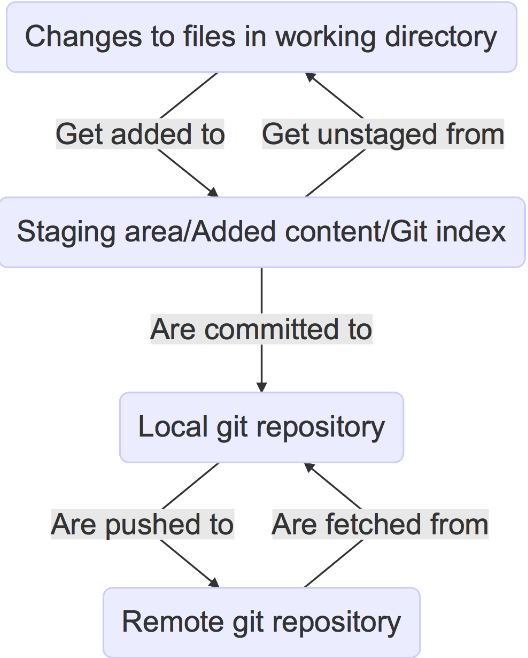
\includegraphics[width=0.3 \linewidth]{Photos/interactive-1.png}
    \caption[short]{The four stages of working in Git}
    \label{fig:interactive-1}
\end{figure}

So far you have been shown the difference between adding (staging) and committing, but this still leaves a lot of room for confusion. What's the point of the seperation between the two? Why not just commit everything?

\section{The Add Interactive command}

The git add -i command is a powerful tool that allows you to interactively add files to the index. It allows you to add files in hunks, which means that you can add parts of a file, rather than the whole file.

\section{The git add -i command}

Let us demonstrate how you might want to use this with a simple example.

\begin{lstlisting}
    mkdir lgthw_add_i
    cd lgthw_add_i
    git init
    echo 'This is file1' > file1
    echo 'This is file2' > file2
    git add file1 file2
    git commit -am 'files added'
    cat > file1 << END
    > Good change
    > This is file1
    > Experimental change
    > END
    cat > file2 << END
    > All good
    > This is file2
    > END
\end{lstlisting}

Now run the following, and input the characters (or just "enter"/"return") at the appropriate points:

\begin{lstlisting}
    git add -i
    What now> p
    Patch update>> 1
\end{lstlisting}

Note that in the next line, you only need to input the "enter"/"return" key. Just hit "return".

\begin{lstlisting}
    Patch update>>
    Stage this hunk [y,n,q,a,d,/,s,e,?]? s
    Stage this hunk [y,n,q,a,d,/,s,e,?]? y
    Stage this hunk [y,n,q,a,d,/,s,e,?]? n
    What now> q
    git status
    git diff
\end{lstlisting}

Now you have staged the good change, but have not lost the other changes you made. This gives you more granular control over the changes committed.

A lot went on in that last block of output so it's worth reading over it carefully.

First, you were presented with a set of choices:

\begin{lstlisting}
    1: status   2: update   3: revert   4: add untracked
    5: patch    6: diff     7: quit     8: help
\end{lstlisting}

\section{Patch}
We're only going to focus on "patch" (number 5) here. There's no point exhaustively listing all the choices and their meanings, as most of them are self-explanatory, and I did not feel the need to use the rest of them.

\section{Hunk}
As you have probably figured out already, a "hunk" is a contiguous (or nearly contiguous) section of a diff.

You're presented with a set of numbered changes. There were files that had changes to them presented to you.

\begin{lstlisting}
            staged     unstaged path
    1:   unchanged        +2/-0 file1
    2:   unchanged        +1/-0 file2
\end{lstlisting}

\section{Staged}
The first "staged" column tells you what has been staged so far.

\section{Unstaged}
The second "unstaged" column tells you how many lines have been added/removed. In the above example, two lines have been added and none removed.

\section{Path}
The third is the "path" of the file.

An asterisk (*) indicates that the option is the chosen one. So by hitting that number, followed by the enter/return key, you only need to further hit the enter/return key once to choose the first hunk. Then you are presented with the hunk itself and a bewildering series of options:

\begin{lstlisting}
    diff --git a/file1 b/file1
    index 6a00e12..014f6e4 100644
    --- a/file1
    +++ b/file1
    @@ -1 +1,3 @@
    +Good change
    This is file 1
    +Experimental change
    Stage this hunk [y,n,q,a,d,/,s,e,?]?
\end{lstlisting}

\section{Splitting}
At this point, you chose s, which stands for "split" the hunk.

If you're not sure what's going on, you can choose the ? option here, which explains what the various options mean. If I'm stuck, I can never remember what they all do, so I depend heavily on ?. Read through the options now, and make sure you understand them all.

Once split, you can "stage" the hunks one at a time by choosing y for "yes" when prompted.

If you are happy with the changes, you can commit all the changes you have made.

\section{Why split hunks?}
Why is this splitting useful? It's most commonly used to avoid committing lines you might want to keep for local development but not persist in the repository history.

A typical example of this is printed debug lines that you don't want to get to production but want to keep for local development. Another example might be chunks of notes that only make sense to you while you are developing.

\section{Why stage at all}
Committing will commit all the changes you have staged. What is the point of staging then? It is to confirm that you want to commit some changes made locally, but not others. These changes are added to the index (as opposed to the repository).

Remember: index == staging == adding

By committing, it commits your staged changes to the local repository (as opposed to adding). After which, these commits can be pushed to remote repositories.

If (like me) you run git commit -am "your commit message" frequently, then you skip over these steps, which can result in commits with stray lines that you would not want to be part of the history.

The -a flag stands for "automatically add". Confusingly, the -a flag is aliased to --all, even though not all files are necessarily added; only the already-added ones are.

\chapter{git reflog}

References to your history in a sequential format. 

<<After updating a few commits to the git project>>

You accidentally:

\begin{lstlisting}
    git checkout HEAD^
    git branch -f master
    git checkout master
    git log
\end{lstlisting}

And you find out that your latest commit has *disappeared*.

You slayed. But badly.

You have fully reverted the master branch to where it was before. Even git log --all does not show it because it's not on a branch.

Retrieve commit
This is where Git's reflog can help.

Git reflog records all movements of branches in the repository. As with git stashes, it is local to your repository.

The reflog is called that because it's a "REFerence LOG".

Git's reflog is a history of the changes made to the HEAD (remember the HEAD is a pointer to the current location of the repository).

\begin{lstlisting}
    git reflog
\end{lstlisting}

To restore state, use git reset.

If you run git reset:

\begin{lstlisting}
root@educative:/lgthw_reflog# git reflog
86f146a HEAD@{0}: checkout: moving from 86f146a8e8eb8f730ee7b090e760d116f2a8f018 to master
86f146a HEAD@{1}: checkout: moving from master to HEAD^
c11d00d HEAD@{2}: commit: second commit message for file1.1
86f146a HEAD@{3}: commit (initial): first commit
\end{lstlisting}
this should be the output.

You are returned to where you were.

The --hard flag updates both the index (staging/added) and the working tree that you saw previously.

The relfog contains references to the state if the repository at various points, even if those points are no longer apparently reachable within the repository.

\chapter{Cherry-picking}

This chapter covers:
\begin{itemize}
    \item git cherry-pick
    \item A revisit of git log
    \item A revisit of git branch
\end{itemize}

\section{Introduction}

Importance of cherry-picking

This chapter is important because cherry-picking is the simplest-to-understand means to move commits around. This is the basis of the more sophisticated movement of commits, such as rebasing and "squashing" commits.

\section{A simple cherry-pick}

\end{document}
